\documentclass[11pt]{article}
\usepackage{latexsym}
\usepackage{amsmath}
\usepackage{amssymb}
\usepackage{amsthm}
\usepackage{epsfig}
\usepackage[tight]{subfigure}
\usepackage{xcolor}

\usepackage{amsmath}

\DeclareMathOperator*{\minimize}{min}
\DeclareMathOperator*{\maximize}{max}

\usepackage{algorithm}
 %on linux you may need to run sudo apt-get install texlive-full to install algorithm.sys
\usepackage{algorithmic}

\usepackage{verbatim}

\newcommand{\handout}[5]{
  \noindent
  \begin{center}
  \framebox{
    \vbox{
      \hbox to 5.78in { {#1} \hfill #2 }
      \vspace{4mm}
      \hbox to 5.78in { {\Large \hfill #5  \hfill} }
      \vspace{2mm}
      \hbox to 5.78in { {\em #3 \hfill #4} }
    }
  }
  \end{center}
  \vspace*{4mm}
}

\newcommand{\lecture}[5]{\handout{#1}{#2}{#3}{#4}{#5}}
\newcommand{\collision}[0]{\mathrm{collision}}
\newcommand{\nocollision}[0]{\overline{\collision}}

\newcommand*{\QED}{\hfill\ensuremath{\square}}

\newtheorem{theorem}{Theorem}
\newtheorem{corollary}[theorem]{Corollary}
\newtheorem{lemma}[theorem]{Lemma}
\newtheorem{observation}[theorem]{Observation}
\newtheorem{proposition}[theorem]{Proposition}
\newtheorem{definition}[theorem]{Definition}
\newtheorem{claim}[theorem]{Claim}
\newtheorem{fact}[theorem]{Fact}
\newtheorem{assumption}[theorem]{Assumption}
\newtheorem{note}[theorem]{Note}

% 1-inch margins, from fullpage.sty by H.Partl, Version 2, Dec. 15, 1988.
\topmargin 0pt
\advance \topmargin by -\headheight
\advance \topmargin by -\headsep
\textheight 8.9in
\oddsidemargin 0pt
\evensidemargin \oddsidemargin
\marginparwidth 0.5in
\textwidth 6.5in

\parindent 0in
\parskip 1.5ex
%\renewcommand{\baselinestretch}{1.25}

\begin{document}

\lecture{Statistical Techniques in Robotics (16-831, S21)}{Lecture \#05
  (Monday, February 15)}{Lecturer: Kris Kitani}{Scribes: Xuhua Huang, Xinjie Yao}{OLC (Perceptron, Winnow)}

\section{Review}
In the last lecture, without the assumption of at least one perfect expert (realizability), we dive into two main algorithms: (1) Weighted Majority Algorithm (WMA), and (2) Random Weighted Majority Algorithm (RWMA) \cite{littlestone1989weighted}.
In this lecture, we will shift to a new topic named Online Linear Classification (OLC). One common feature between OLC and WMA is that they only have access to a subset of states, so they are both sampled learning. We will introduce and analyze two approaches to learn an online linear classifier: Perceptron Algorithm \cite{rosenblatt_1958} and Winnow Algorithm  \cite{Winnowlittlestone}. As a high-level takeaway, both of them will construct a linear classifier on-the-fly, while the key differences are: (1) weight update rules (additive updates vs. multiplicative updates) (2) prediction function (hyperplane classifier vs. disjunctive boolean function). Before jumping into these two algorithms, we will recap WMA and RWMA together with a few definitions to understand the regret bound. Then, we will introduce the context of online linear classifiers with their problem setup. 
% In this lecture, we will introduce and analyze two more algorithms for the PWEA problem, namely: the Weighted Majority Algorithm (WMA) and the Randomized Weighted Majority Algorithm (RWMA). For a quick high level takeaway, we note that the Weighted Majority Algorithm (WMA) has a bounded regret, while the RWMA is our first no regret algorithm. This lecture, after the review section, will derive these results. In the next two subsections, we first recap the problem of prediction with expert advice and a few definitions to help us along the way in deriving those results.

%This section serves as a review of the previous lecture and any other context required to frame the content of the current lecture. 

%You may format the scribes in any way you like, aside from changing font style, size and page format. Please use subsections and paragraphs to increase the readability of your notes.

%Length requirement 1-2 pages.
        
\subsection{Weighted Majority Algorithm(WMA)}
WMA makes learner prediction based on a sum of weighted experts and updates those weights with a penalty parameter $\eta$. Specifically, the prediction rule and weight update rule are as follows,
\begin{align}
\hat{y}^{(t)} = \text{sign}\Big(\sum_{n=1}^Nx_n^{(t)}\cdot w_n^{(t)}\Big)\in\{-1, 1\} \\
w_n^{(t+1)}\leftarrow w_n^{(t)}\big(1-\eta\cdot\textbf{1}[y^{(t)}\neq x_n^{(t)}]\big)
\end{align}
Since there is no prefect expert in this setup, we utilize regret of the learner, $R^{(T)}(H)$, a cumulative loss for not following the best hypothesis in the hypothesis class $H$. The regret is proved to be bounded by
\begin{align}
    R(h_n) = M^{(T)} - m_n^{(T)} \leq (1+2\eta) m_n^{(T)} + \frac{2\log N}{\eta}
\end{align}
We observe that WMA has bounded regret with the upper bound grow linear over time. however, it is \textit{NOT} a no-regret algorithm. The upper bound of average regret over time can't converge to 0 as $T\rightarrow\infty$.  
\subsection{Random Weighted Majority Algorithm(RWMA)}
By adding some randomization, we demonstrate it in RWMA that the number of mistakes will be cut by a half. Also, it turns out to be a no-regret algorithm. Specifically, the learner makes prediction by sampling from a multinomial distribution of the weights. 
\begin{align}
h&\sim \textsc{Multinomial}(\textbf{w}^{(t)}/\Phi^{(t)})\text{, where } \Phi^{(t)}=\sum_{n=1}^Nw_n^{(t)} \nonumber \\
\hat{y}^{(t)}&=h_i(\textbf{x}^{(t)})
\end{align}
By only modifying the prediction rule, RWMA could yield a much better performance. The expected regret is further bounded by, 
\begin{align}
    \mathbb{E}[R] \leq \eta m_n^{(T)} + \frac{\log N}{\eta}
\end{align}
If we set $\eta=\frac{1}{\sqrt{T}}$, 
% $\mathbb{E}[R]= \Big(\eta m_n^{(T)} + \frac{\log N}{\eta}\Big) \propto \frac{1}{\sqrt{T}}$; $\frac{\mathbb{E}[R]}{T}\rightarrow 0\;\text{as}\;T\rightarrow\infty$. 
it turns out RWMA is a no-regret algorithm.

% \subsection{Introduction}
% \textcolor{blue}{@xuhua: history of OLC}
% Linear Classification tries to learn a linear predictor function, where the decision boundary is a hyperplane defined by a set of weights. With the rapid development of society, lots of heavy and repetitive classification tasks are waiting to be carried by an autonomous system. However, due to the large volume of data and the constantly changing classification criteria in production environment, it is impossible to learn an linear predictor function offline. This is why Online Learning Classification comes into play. In Online Learning Classification, the linear predictor function can evolve on-the-fly, and over time it is able to converge to the performance of an expert. In following sections we will dive into two representative algorithms to learn a linear classifier online.

\section{Summary}

\subsection{Perceptron Algorithm}
Now we will start with the first algorithm - Perceptron algorithm, in Online Linear Classification (OLC). The algorithm details are listed as Algorithm \ref{algo:perceptron} below. It is worthy of attention that, the perceptron algorithm makes prediction based on a sign function (line 4), and it applies an additive update after receiving answer from nature (line 6). These are the two major differences compared with Winnow algorithm introduced in Section \ref{section:winnow}.
\begin{algorithm}[H]
\caption{Perceptron algorithm}
\label{algo:perceptron}
\begin{algorithmic}[1]
\STATE $\textbf{w}^{(1)} \leftarrow 0$ \hfill $\triangleright$ Weight initialization
\FOR{$t=1,\;\cdots,\;T$}
\STATE \textsc{Receive} ($\textbf{x}^{(t)}\in \mathbb{R}^N$) \hfill $\triangleright$ Receive expert predictions
\STATE $\hat{y}^{(t)} = \text{sign}\Big(\langle \textbf{w}^{(t)}, \textbf{x}^{(t)}\rangle \Big)$ \hfill $\triangleright$ Make learner prediction
\STATE \textsc{Receive} ($y^{(t)}\in\{-1, 1\}$) \hfill $\triangleright$ Receive actual answer
\STATE $\textbf{w}^{(t+1)}\leftarrow \textbf{w}^{(t)} + y^{(t)} \cdot \textbf{x}^{(t)} \cdot\textbf{1}[y^{(t)}\neq \hat{y}^{(t)}] $ \hfill $\triangleright$ Weight update
\ENDFOR
\end{algorithmic}
\end{algorithm}

There are some characteristics of perceptron algorithm:
\begin{itemize}
\item It is fast. Because the prediction function is a dot product, and the update is just a sum, simple computation is involved.
\item It is \textbf{not} a large margin classifier. It only uses sign to make decision, so there is no notion of margin in the algorithm. 
\item It does \textbf{not} work for non-separable data. The decision boundary of perceptron algorithm is defined by a linear hyperplanes, so it only works when data is linearly separable. 
\end{itemize}

Now we will derive the mistake bound below, and before that we will recap a lemma about dot product.

\lemma{The dot product of two vectors is largest when they are parallel.}\label{lemma:dotproduct}

\theorem{ (Perceptron Mistake Bound) Let R be the norm of observations, $R=\max\limits_t \|x^{(t)}\|$, and $\gamma$ be the margin of separability, $\gamma=\min\limits_t y_t \langle \textbf{w}^\star, \textbf{x}^{(t)} \rangle $ where $\|\textbf{w}^\star\|=1$, the Perceptron mistake is bounded as follows,
$$
    M \leq \frac{R^2}{\gamma^2}
$$

\proof{Let's define the potential function as the squared $l_2$ norm of weight vector by, 
\begin{align}
    \Phi(t) &= \| \textbf{w}^{(t)}\|^2 = \sum_n (w_n^{(t)})^2 \nonumber \\
    &= \| \textbf{w}^{(t-1)}+ y^{(t)} \cdot \textbf{x}^{(t)}\| ^2 \;\;\;\text{(where a mistake is made)} \nonumber \\
    &= \| \textbf{w}^{(t-1)}\|^2 + \| \textbf{x}^{(t)} \|^2 +2y^{(t)}\langle \textbf{w}^{(t-1)}, \textbf{x}^{(t)}\rangle 
    \nonumber \\
    &\leq \| \textbf{w}^{(t-1)}\|^2 + \| \textbf{x}^{(t)} \|^2
    \;\;\;\because (y^{(t)}\langle \textbf{w}^{(t-1)}, \textbf{x}^{(t)}\rangle <0 \text{ if a mistake)} \nonumber \\
    &\leq  \| \textbf{w}^{(t-1)}\|^2+R^2 
    \;\;\; \text{(Recall } R=\max\limits_t \|x^{(t)}\| )
    \label{eq:PerceptronPotentialUpper}
\end{align}

By induction to the base case using Eq. \ref{eq:PerceptronPotentialUpper}, one can conclude the potential function is upper bounded by,
\begin{align}
    \Phi(t) \leq \| \textbf{w}^{(0)}\|^2 + M^{(T)}\cdot R^2 =  M^{(T)}\cdot R^2 \;\;\; (M^{(T)} \text{ is the number of mistakes)}
    \label{perceptronpotentialupper}
\end{align}
We have upper-bounded the potential function, now let's derive the lower bound with an intermediate potential function,
\begin{align}
    \left\langle\boldsymbol{w}^{*}, \boldsymbol{w}^{(t)}\right\rangle
    \label{eq:dot}
\end{align}
Here, $\boldsymbol{w}^{*}$ denotes a perfect classifier, whose norm is required to be 1 (i.e. unit vector), and $\boldsymbol{w}$ denotes our classifier at time step $t$. We will start by deriving the upper bound and lower bound of this dot product.

\underline{Upper bound}:

From Lemma \ref{lemma:dotproduct}, we know Eq. \ref{eq:dot} becomes largest when $\boldsymbol{w}^{*}$ equals to the unit vector oriented in the same direction as $\boldsymbol{w}$, stated as:
\begin{align}
    \frac{\boldsymbol{w}}{\|\boldsymbol{w}\|}=\underset{\boldsymbol{w}^{\prime}}{\arg \max }\left\langle\boldsymbol{w}^{\prime},     \boldsymbol{w}\right\rangle
\end{align}

Because $\boldsymbol{w}^{*}$ is also a unit vector, so the dot product of Eq. \ref{eq:dot} will satisfy this inequality, 
\begin{align}
    \left\langle\boldsymbol{w}^{*}, \boldsymbol{w}^{(T)}\right\rangle \ \leq\left\langle\frac{\boldsymbol{w}^{(T)}}{\left\|\boldsymbol{w}^{(T)}\right\|}, \boldsymbol{w}^{(T)}\right\rangle=\frac{\left\|\boldsymbol{w}^{(T)}\right\|^{2}}{\left\|\boldsymbol{w}^{(T)}\right\|}=\left\|\boldsymbol{w}^{(T)}\right\|
    \label{eq:11}
\end{align}

Therefore, Eq. \ref{eq:dot} is upper-bounded by the norm of the hyperplane $\boldsymbol{w}$ at time step $t$.

\underline{Lower bound}:

Let's recap the weights $\boldsymbol{w}$ update rule at each time step $t$ here, 
\begin{align}
    \textbf{w}^{(t)} = \textbf{w}^{(t-1)} + y^{(t)} \cdot \textbf{x}^{(t)} \cdot\textbf{1}[y^{(t)}\neq \hat{y}^{(t)}]
\end{align}
By applying dot product with perfect classifier $\boldsymbol{w}^{*}$ on both side, we can get,
\begin{align}
    \left\langle\boldsymbol{w}^{*}, \boldsymbol{w}^{(t)}\right\rangle 
    &= \left\langle\boldsymbol{w}^{*}, \boldsymbol{w}^{(t-1)}\right\rangle + y^{(t)}\left\langle\boldsymbol{w}^{*}, \boldsymbol{x}^{(t)}\cdot\textbf{1}[y^{(t)}\neq \hat{y}^{(t)}]\right\rangle \nonumber\\ 
    &= \left\langle\boldsymbol{w}^{*}, \boldsymbol{w}^{(t-1)}\right\rangle+y^{(t)}\left\langle\boldsymbol{w}^{*}, \boldsymbol{x}^{(t)}\right\rangle \;\;\;(\because \text{perfect classifier make no mistake)} \nonumber\\
    &\geq \left\langle\boldsymbol{w}^{*}, \boldsymbol{w}^{(t-1)}\right\rangle + \gamma \text{, where } \gamma=\min _{t} y_{t}\left(\boldsymbol{w}^{*}, \boldsymbol{x}^{(t)}\right\rangle
\end{align}

Because $y^{(t)}\left\langle\boldsymbol{w}^{*}, \boldsymbol{x}^{(t)}\right\rangle$ denotes the distance from each data points to the hyperplane and $\gamma$ is the margin, which is the smallest distance among all points.

By induction starting from based case $t = 0$, 
\begin{align}
    \left\langle\boldsymbol{w}^{*}, \boldsymbol{w}^{(1)}\right\rangle \geq\left\langle\boldsymbol{w}^{*}, \boldsymbol{w}^{(0)}\right\rangle+\gamma
\end{align}

We can add a single $\gamma$ on RHS at each time step and reach, 
\begin{align}
    \left\langle\boldsymbol{w}^{*}, \boldsymbol{w}^{(T)}\right\rangle &\geq\left\langle\boldsymbol{w}^{*}, \boldsymbol{w}^{(0)}\right\rangle + M^{T}\cdot\gamma \nonumber \\ 
    &= M^{T} \cdot \gamma \;\;\;(\because \boldsymbol{w}  \text{ is initialized to 0 at } t=0)
    \label{eq:15}
\end{align}

\underline{Combine}:

Now we have got the upper bound of Eq. \ref{eq:dot} from Eq. \ref{eq:11} and the lower bound from Eq.  \ref{eq:15}. By combing, 

\begin{align}
    M^{T} \cdot \gamma \leq 
    \left\langle\boldsymbol{w}^{*}, \boldsymbol{w}^{(T)}\right\rangle
    \leq \left\|\boldsymbol{w}^{(T)}\right\|
\end{align}

We have,
\begin{align}
     M^{T} \cdot \gamma \leq \left\|\boldsymbol{w}^{(T)}\right\|
\end{align}

The above equation still holds when we apply a power of 2 for both sides, and we get,
\begin{align}
     {(M^{T} \cdot \gamma)}^{2} \leq {\left\|\boldsymbol{w}^{(T)}\right\|}^{2} \text { , where } {\left\|\boldsymbol{w}^{(T)}\right\|}^{2} \text{is our defined potential function}
     \label{eq:18}
\end{align}
}

Now that we have successfully derived the upper bound and lower bound of potential function in Eq. \ref{perceptronpotentialupper} and Eq. \ref{eq:18}, we can combine both to get the mistake bound of Perceptron,
\begin{align}
    {(M^{T} \cdot \gamma)}^{2} &\leq 
    M^{(T)}\cdot R^2 \nonumber \\
    \therefore M^{(T)} &\leq \frac{R^{2}}{\gamma^{2}}
 \end{align}

}



% Winnow 
\subsection{Winnow Algorithm}
\label{section:winnow}
\normalfont Now we will introduce the second algorithm in OLC, named Winnow algorithm. Winnow assumes only a subset of features are relevant for classification. Its predictor (line 4) works as a disjunction function, trying to learn set of weights on relevant features and make sum greater than N on positive examples. The weight update rule (line 6) is multiplicative.

\begin{algorithm}[H]
\caption{Winnow algorithm}
\label{algo:perceptron}
\begin{algorithmic}[1]
\STATE $\textbf{w}^{(1)} \leftarrow \{1,...,1\}$ \hfill $\triangleright$ Weight initialization
\FOR{$t=1,\;\cdots,\;T$}
\STATE \textsc{Receive} ($\textbf{x}^{(t)} \in\{0, 1\}^N$) \hfill $\triangleright$ Receive expert predictions
\STATE $\hat{y}^{(t)} = \textbf{1}[\langle \textbf w^{(t)}, \textbf x^{(t)}\rangle>N]$ \hfill $\triangleright$ Make learner prediction
\STATE \textsc{Receive} ($y^{(t)}\in\{0, 1\}$) \hfill $\triangleright$ Receive actual answer
\STATE $w_n^{(t+1)}\leftarrow w_n^{(t)} (1+\beta)^{ (y^{(t)}-\hat{y}^{(t)})\cdot x_n^{(t)}} $ \hfill $\triangleright$ Weight update
\ENDFOR
\end{algorithmic}\label{algo:winnow}
\end{algorithm}

% Derive mistake bound 
\normalfont
Different from perceptron where weight decays, Winnow could increase or decrease weight depending on the type of mistake. Recall the weight update rule (line 7 in Algorithm \ref{algo:winnow}),  
\begin{align}
w_n^{(t+1)}\leftarrow w_n^{(t)} (1+\beta)^{ (y^{(t)}-\hat{y}^{(t)})\cdot x_n^{(t)}} 
\end{align}
It shows that making a mistake on a positive example brings different gain to weights of relevant features than making a mistake on a negative example. The weight update rule is summarized in the following table. 
% if making a mistake on a positive example, where $\hat{y}^{(t)}=0$ (prediction) and ${y}^{(t)}=1$ (example), weights on relevant features will be increased by $(1+\beta)^{({y}^{(t)}-\hat{y}^{(t)})}=(1+\beta)$. Similarly, if making a mistake on a negative example, where $\hat{y}^{(t)}=1$ (prediction) and ${y}^{(t)}=0$ (example), weights on relevant features will be decreased by $(1+\beta)^{({y}^{(t)}-\hat{y}^{(t)})}=\frac{1}{(1+\beta)}$.
\begin{table}[!htbp]
\centering
\begin{tabular}{|c|c|c|c|c|}
\hline
True ($y^{(t)}$) & Prediction ($\hat{y}^{(t)}$) & Type of mistake     & Gain (${y}^{(t)}-\hat{y}^{(t)}$) & Weight update \\ \hline
0    & 1          & mistake on negative & -1   & decrease by $\frac{1}{(1+\beta)}$   \\ \hline
1    & 0          & mistake on positive & 1    & increase by  $(1+\beta)$ \\ \hline
\end{tabular}
\caption{\label{tab:Weight Update}Winnow updates weights depending on the type of mistake.}
\end{table}

\lemma{Assume there is a relevant feature whose index is $n$, and its weight is $w^t_n$. After $m$ mistakes on positive, its weight will be, 
\begin{align}
    w^t_n = (1+\beta)^m \nonumber
\end{align}
\proof{
Recap on the weights update rule,
\begin{align}
    w_n^{(t+1)} &=  w_n^{(t)} (1+\beta)^{ (y^{(t)}-\hat{y}^{(t)})\cdot x_n^{(t)}} \nonumber \\
    &=  w_n^{(t)} (1+\beta)^{x_n^{(t)}} \;\;\;( \because (y^{(t)}-\hat{y}^{(t)}) = 1 \text{ when mistake on positive)}
\end{align}
For a relevant feature, it will always be true in each time step $t$, which means $x_n^{(t)} = 1$ is held in every weight update step. Therefore, by induction we can get, 
\begin{align}
    w^t_n = (1+\beta)^m \nonumber
\end{align}
}
\label{lemma:3}
}

\lemma{Assume there is a relevant feature whose index is $n$, and its weight is $w^t_n$. Making a mistake on a positive example, 
\begin{align}
    w_{n}^{(t)}<N \quad \forall n \nonumber
\end{align}
\proof{
When we are making mistake on positive, it implies that the ground truth label $y^{(t)} = 1$ and our predicted label $\hat{y}^{(t)} = 0$. Let's look back to our predictor function (line 4 in Algorithm  \ref{algo:winnow}), it is only possible to output $\hat{y}^{(t)} = 0$ when and only when, 
\begin{align}
  \langle \textbf w^{(t)}, \textbf x^{(t)}\rangle < N  \label{eq:wxleqn}
\end{align}
From the proof of Lemma \ref{lemma:3} we have already known $\textbf x^{(t)}_n$ is always 1 (i.e. true) for relevant features. If we assume  $w_{n}^{(t)} > N$, we can derive that $\langle \textbf w^{(t)}, \textbf x^{(t)}\rangle > N$, which contradicts Eq. \ref{eq:wxleqn}. Therefore, 
\begin{align}
    w_{n}^{(t)}<N \quad \forall n \nonumber
\end{align}
}\label{lemma:4}
}
%mistake bound
\theorem{(Mistake bound of Winnow) Let $M$ be the total number of mistakes made by the learner, and $k$, $N$ respectively be the number of relevant features and the total number of features. Assuming $\beta=1$, then $M$ is upper-bounded as:
$$
M<2+3k(log_2 N+1)
$$\label{theorem:WinnowBound}
}%define potential

\proof{Let's define the potential function for Winnow as the sum of weights among all features, 
\begin{align}
  \Phi^{(t)} = \sum_{n=1}^N w_n^{(t)} \label{eq:WinnowPotential} 
\end{align}


Note that the total mistakes, $m$, consist of mistakes on positive examples $m^+$, and mistakes on negative examples $m^-$. Since weight update rules depend on types of mistakes, we handle each case separately to bound the potential function. $$
m = m^+ + m^-
$$
We will starts with mistakes on positive examples. Following the weight update rule of Winnow in Table.\ref{tab:Weight Update}, $w_n^{(t)}=(1+\beta)w_n^{(t-1)}=2w_n^{(t-1)}$. It doubles the weights on relevant features where $x_n^{(t-1)}=1$. Thus, we can derive the mathematical relation between $\Phi^{(t)}$ and $\Phi^{(t-1)}$ as follows:
\begin{align}
    \Phi^{(t)} = \Phi^{(t-1)} + \sum_{n:x_n^{(t)}=1} w_n^{(t-1)} \nonumber\\
    = \Phi^{(t-1)} + \textbf{w}^{(t-1)}\cdot \textbf{x}^{(t-1)}\label{eq:PositiveUpdate}
\end{align}
\underline{Upper bound}:

Recall the prediction rule in Algorithm \ref{algo:winnow} (line 5), making a mistake on a positive example means $\hat{y}^{(t)}=\textbf{1}[\langle \textbf w^{(t)}, \textbf x^{(t)}\rangle>N]=0$. In other words, $\textbf{w}^{(t-1)}\cdot \textbf{x}^{(t-1)} \leq N$. By substituting it into Eq. \ref{eq:PositiveUpdate}, the mathematical relation between $\Phi^{(t)}$ and $\Phi^{(t-1)}$ could be constrained by, 
\begin{align}
    \Phi^{(t)} \leq \Phi^{(t-1)} +N \label{eq:PositiveUpdateBaseCase}
\end{align}
By induction to relate the base case using Eq. \ref{eq:PositiveUpdateBaseCase}, the upper bound on potential from mistakes on positive examples is as follows:
\begin{align}
    \Phi^{(t)} \leq \Phi^{1} + m^+N = N + m^+N \label{eq:PositiveUpdateUpper}
\end{align}

Now we take a look at the mistakes on negative examples. Instead of increasing weights when making mistakes on positive examples, Eq. \ref{eq:PositiveUpdate} becomes as follows:
\begin{align}
    \Phi^{(t)} = \Phi^{(t-1)} - \sum_{n:x_n^{(t)}=1} \frac{1}{2}w_n^{(t-1)} \nonumber\\
    = \Phi^{(t-1)} - \frac{1}{2} \textbf{w}^{(t-1)}\cdot \textbf{x}^{(t-1)}\label{eq:NegativeUpdate}
\end{align}

Similarly, making a mistake on a negative example means 
 $\hat{y}^{(t)}=\textbf{1}[\langle \textbf w^{(t)}, \textbf x^{(t)}\rangle>N]=1$. In other words, $\textbf{w}^{(t-1)}\cdot \textbf{x}^{(t-1)} > N$. By substituting it into Eq. \ref{eq:NegativeUpdate}, the mathematical relation between $\Phi^{(t)}$ and $\Phi^{(t-1)}$ could be constrained by, 
\begin{align}
    \Phi^{(t)} < \Phi^{(t-1)} -\frac{1}{2}N \label{eq:NegativeUpdateBaseCase}
\end{align}
By induction to relate the base case using Eq.\ref{eq:NegativeUpdateBaseCase}, the upper bound on potential from mistakes on positive examples is as follows:
\begin{align}
    \Phi^{(t)} < \Phi^{1} -\frac{1}{2}m^-N = N - m^-\frac{1}{2}N \label{eq:NegativeUpdateUpper}
\end{align}

Combining penalty from positive mistakes Eq.\ref{eq:PositiveUpdateUpper} and penalty from negative mistakes Eq.\ref{eq:NegativeUpdateUpper}, the potential is upper-bounded by 
\begin{align}
    \Phi^{(t)} \leq N +m^+N - m^-\frac{1}{2}N \label{eq:WinnowPotentialUpper}
\end{align}
\underline{Lower bound}:

Next, as weights are initialized to 1 and sign never change during updates, one can conclude the potential is lower-bounded by,
\begin{align}
    0 < \Phi^{(t)} \label{eq:WinnowPotentialLower}
\end{align}
\underline{Combine}:

Then, by combining the upper bound Eq.\ref{eq:WinnowPotentialUpper} and lower bound Eq.\ref{eq:WinnowPotentialLower}, the potential is bounded as follows,
\begin{align}
    0 < \Phi^{(t)} \leq N +m^+N - m^-\frac{1}{2}N
    \label{eq:WinnowPotentialCombine}
\end{align}

% \textcolor{blue}{@xuhua: from potential to mistake bound}
Though we have bounded our potential function, but what we really want is to bound the total mistakes $M$ defined below, and now we are going to derive the bound of $M$,
\begin{align}
    M = m^+ + m^-
\end{align}

With simple algebra on Eq. \ref{eq:WinnowPotentialCombine}, we get, 
\begin{align}
    N+m^{+} N-m^{-} \frac{1}{2} N &> 0 \nonumber\\
    N+m^{+} N &> m^{-} \frac{N}{2} \;\;\;(\because \text{moving items}) \nonumber \\
    2+2 m^{+} &> m^{-}
    \label{eq:34}
\end{align}

From Lemma \ref{lemma:3}, if $m^+$ mistakes are required for doing correct positive classification, and assuming $\beta=1$, we have,
\begin{align}
    w^t_n = (1+\beta)^m = 2^{(m^+ - 1)}
\end{align}

Combining Lemma \ref{lemma:4}, we have, for a single relevant feature $n$, 
\begin{align}
    w^t_n = 2^{(m^+ - 1)} &< N \nonumber \\
    2^{(m^+ - 1)} &< N \nonumber \\
    m^{+}-1 &< \log _{2} N \nonumber \;\;\; (\because \text{log 2 base on both sides}) \\
    m^{+} &< \log _{2} N+1 \;\;\; (\because \text{algebra})
\end{align}

For $k$ relevant features, we will have,
\begin{align}
    m^{+} &< k(\log _{2} N+1)
\end{align}

With Eq. \ref{eq:34}, we can bound the mistakes on negative $m^-$ by $m^+$, 
\begin{align}
    m^{-} &< 2 + 2m^{+} \nonumber \\
     &= 2 + 2k(\log _{2} N+1)
\end{align}

So the total mistakes $M$, with k relevant features and N totoal number of features, 
\begin{align}
    M &= m^{-} + m^{+} \nonumber \\
      &< 2 + 2k(\log _{2} N+1) + k(\log _{2} N+1)  \nonumber \\
      &= 2 + 3k(\log _{2} N+1)
\end{align}
}

\subsection{Conclusion}
Online Linear Classification problem aims to learn a good linear classifier over time, by feeding correct classification answer from side-by-side experts. It is expected to converge to the performance of the expert ultimately. Therefore, it is suitable for situation where data volume is too huge to train in one batch or the classification criteria is evolving. To solve these problem, we introduce two online linear classification algorithms called Perceptron and Winnow. Both of them involve a linear hyperplane, while Perceptron predicts with sign function and Winnow predicts with logical OR function based on relevant features. Noteworthy, their number of mistakes can be bounded when assuming linear separability of data.


\section{Appendix}
\subsection{ History of Perceptron Algorithm}
\underline{Initial wave of excitement:}

According an article published by The New Yorker in 1958 \cite{NWY}, people were excited by how powerful this perceptron algorithm could be. It was successfully simulated a new electronic brain on IBM 704 computer by Dr. Frank Rosenblatt, and later was implemented as custom hardware consisting of 400 photocells for vision applications \cite{IBM}. Dr. Rosenblatt described it as the first non-biological object which is able to interact with its environments and to compose concepts which have not been accessible for a human agent. It essentially tells the different between a dog and a cat without the ability to locate the dog relative to the position of the cat.  Dr. Rosenblatt was so positive about its promising future that it may be applicable for space exploration \cite{rosenblatt_1958}. 

\underline{Famous XOR problem:}

Then the excitement was hitted by the AI winter. In the book written by Marvin Minsky and Seymour Papert and published in 1969 \cite{minsky69perceptrons}, major limitations for this perceptron algorithm were pointed out. One of the most famous counter-examples is the XOR problem shown in Figure \ref{fig:xor}. Since the data is non-separable, a single layer perceptron can't come in place. 


\begin{figure}[h]
\centering
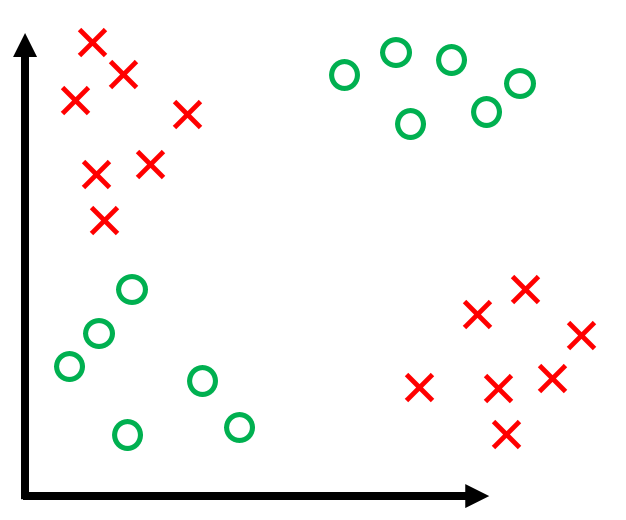
\includegraphics[width=0.4\textwidth]{perceptron_xor.png}
\caption{Illustration of a non-linearly separable data set}
\label{fig:xor}
\end{figure}


\subsection{Comparision between Perceptron and Winnow}

From source \cite{jkivinen_1997}, we can do comparision between Perceptron and Winnow algorithm by the total number of mistakes along trials. In Figure \ref{fig:comp}, $N$ represents the total number of variables / features, and we fix $k = 20$ (i.e. 20 relevant features) in the experiments. The graph shows how the number of mistakes are made in different trials. 

\begin{figure}[h]
\centering
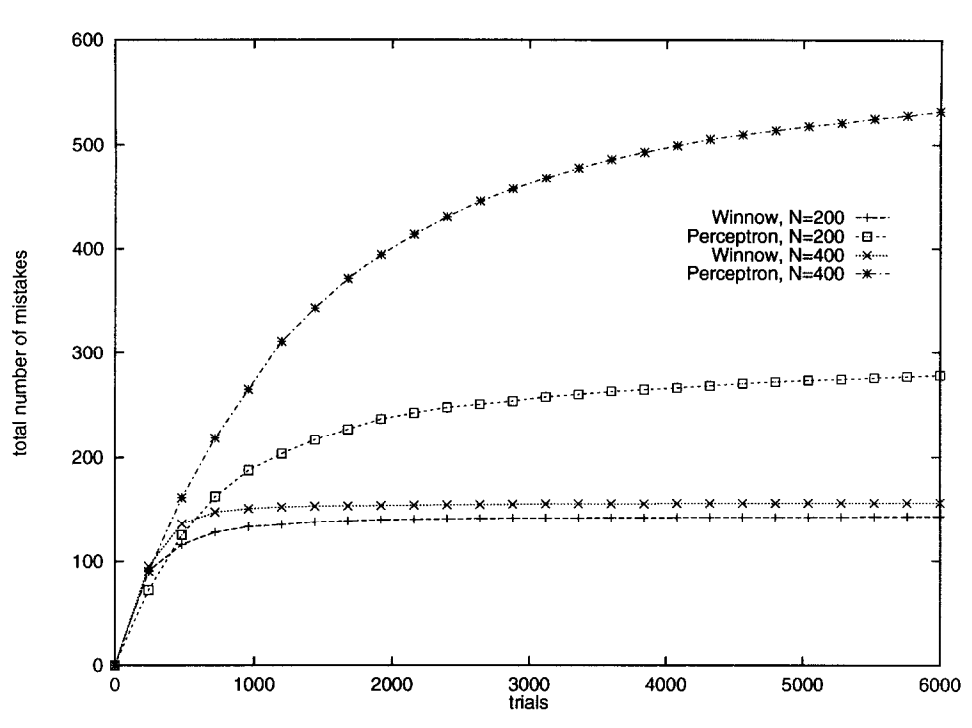
\includegraphics[width=1.0\textwidth]{compare.png}
\caption{Cumulative mistake counts for Winnow and Perceptron algorithm}
\label{fig:comp}
\end{figure}

We notice that Perceptron algorithm is more sensitive to the number of features $N$, if we compared across $N=200$ and $N=400$. However, this change has little effect on Winnow. This may because Winnow algorithm is making prediction on relevant features only. Also, we can clearly notice a convergence trend for both algorithms in this graph, which matches our conclusion in Sec. 2.3.


%\section*{References}
%Include your references here. Please cite any resources you found useful.	
%Populate the refs.bib file or list your references manually. Be consistent in formatting!
{
\bibliography{refs}
\bibliographystyle{abbrv}
}

%\section{Appendix}
%This section provides any relevant background material that was not covered in the lectures, but was found to be useful for understanding the material. 
%For example, derivations, theory underlying techniques employed, etc. 

%Additionally, this section can summarizes applications or extensions of these techniques found in the literature. 

\end{document} % Done!


